\documentclass[a4paper, 11pt]{article}

\usepackage[british]{babel}
\usepackage[autostyle]{csquotes}
\usepackage[colorlinks=true, urlcolor=blue, citecolor=blue]{hyperref}
\usepackage{graphicx}
\usepackage{float}

\graphicspath{{images/}}

\begin{document}

\title{Forecasting Prices Using Stock Market Index Data}
\author{Student Number: 690065435}
\date{December 2022}
\maketitle

\section{Introduction}
Stock markets from across the world are tracked using indices that measure a section of the stock market, such as the Nasdaq Composite Index. Price forecasting is a very important task in the financial industry, as it can be used to guide strategies.

In this project, I propose the following question: can we use regression models on stock market index data to forecast prices effectively? My initial hypothesis is that this is not possible as the stock market is a complex system that is difficult to predict, but we will be able to predict general trends. I will explore the stock exchange dataset, describe our methodology, train three regression models, and discuss the outcomes.

Historically, financial institutions have used discretionary methods to make investment decisions -- they rely on fundamentals and the judgement of analysts \cite{harvey2017man}. However, with the rise of big data and computational power, systematic methods have become increasingly popular -- institutions use rules-based strategies that are implemented by a computer and involve little to no human intervention \cite{harvey2017man}. Systematic methods enable decisions to be made quickly, which leading market makers and high-frequency trading firms such as Jane Street Capital and Hudson River Trading use to exploit arbitrage opportunities and maximise profits by trading at high volumes \cite{aldridge2013high}. However, these firms do not publicly disclose their strategies, which makes it difficult to understand how they make decisions.

Previous studies have investigated the prediction of stock market trends with regression on moving averages \cite{dinesh2021prediction}, but they have focused on individual stocks whereas I am focusing on a stock market index. This is a potential snag, as the index is not a direct representation of the stocks it tracks. The efficient market hypothesis also suggests that this will be difficult, as it states that asset prices reflect all available information, yet we would only be predicting according to a subset of information \cite{fama1970efficient}. 

\section{Methodology and Dataset}

\subsection{About Stock Exchange Dataset}
We are using a \href{https://www.kaggle.com/datasets/mattiuzc/stock-exchange-data}{stock exchange dataset on Kaggle} that was collected from Yahoo Finance and contains the daily price data for stock market indices across the world. Each record in the CSV file contains the following information for each trading day:

\begin{itemize}
    \setlength\itemsep{0em}
    \item Index
    \item Date
    \item Opening price
    \item Highest price 
    \item Lowest price 
    \item Closing price adjusted for splits
    \item Adjusted closing price adjusted for both dividends and splits
    \item Volume of shares traded 
\end{itemize}

\subsection{Data Cleaning}
I loaded the CSV file into a pandas dataframe and converted the date to a datetime64 object to make it easier to work with. It originally consisted of 112457 rows. After looking at the information of the data, I noticed that there were 2204 incomplete rows, so I removed them to ensure that the data was consistent. There were also rows with trading volume recorded as 0 in earlier dates where this information was not available, so I removed them to prevent them from skewing the distribution of volume data -- this further reduced the dataset from 110253 rows to 68160 rows.

\subsection{Data Exploration}
The dataset contains a separate CSV file that describes the index information. I loaded this into a pandas dataframe to see the stock exchange that each index corresponds to. Then, I split the data by index, as each index has different characteristics and may behave differently, and calculated the sample size for each index. I decided to focus on the Nasdaq Composite Index (IXIC) as it has the most data points.

\begin{figure}[H]
    \begin{center}
        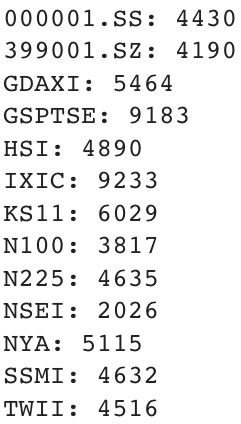
\includegraphics[width=0.2\textwidth]{Sample Size Per Index.png}
        \caption{Sample Size Per Index in Dataset}
    \end{center}
\end{figure}

Next, I calculated the distribution of features to understand patterns in the data. The distributions of open, high, low, close, and adjusted close are extremely similar, as demonstrated in the histograms -- this makes sense as open, close, and adjusted close are between the low and high for each day.

\begin{figure}[H]
    \begin{center}
        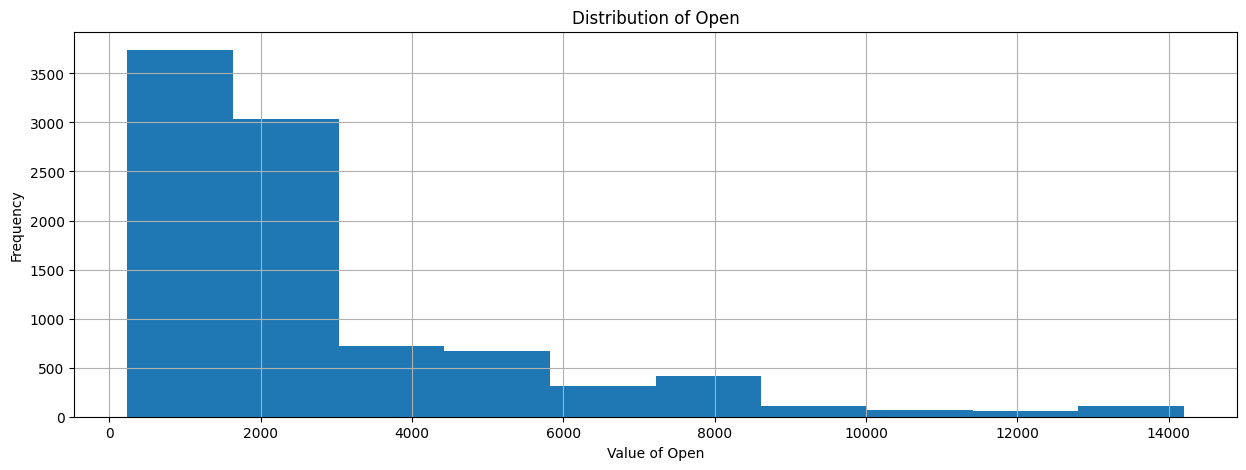
\includegraphics[width=1\textwidth]{Distribution of Open.png}
        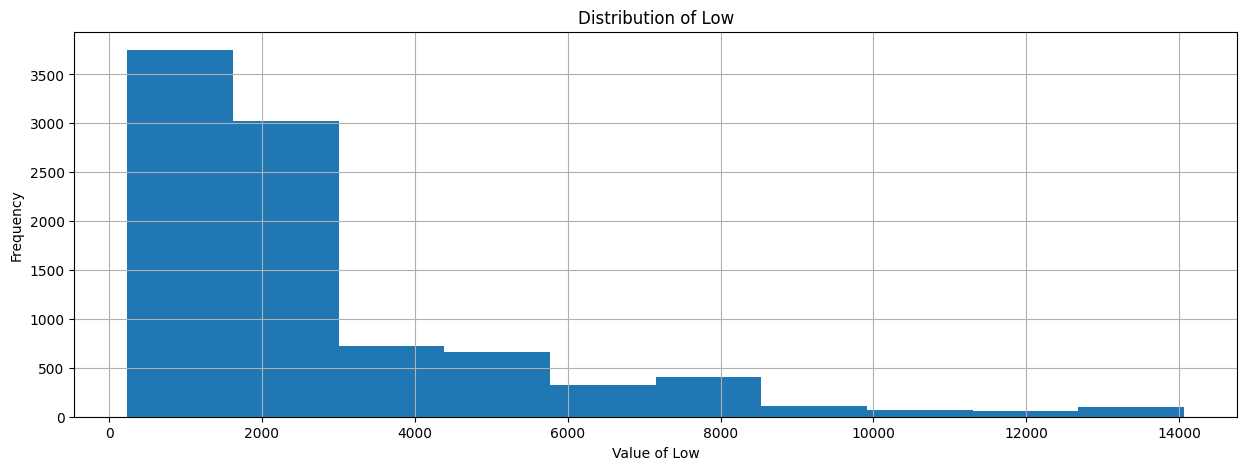
\includegraphics[width=1\textwidth]{Distribution of Low.png}
        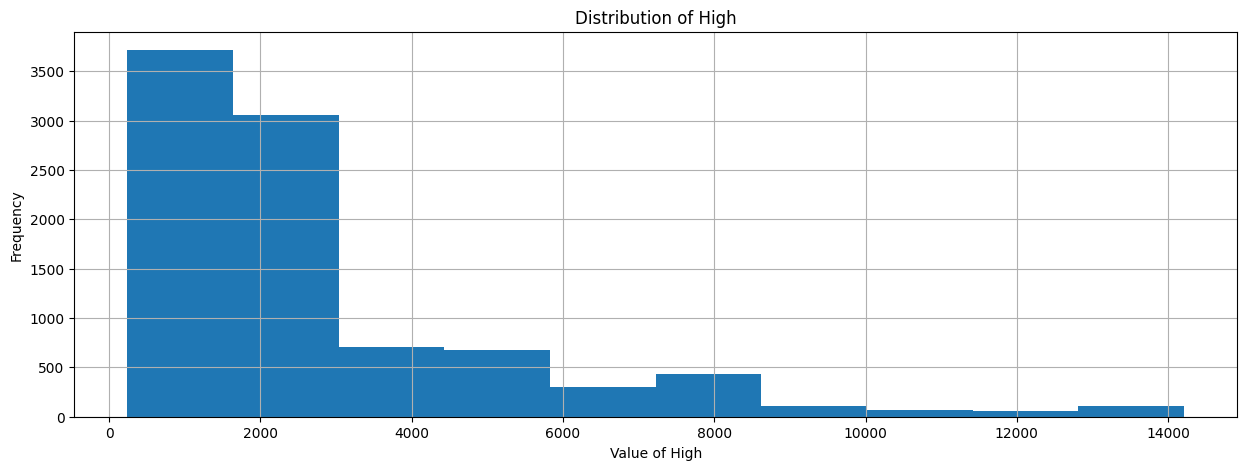
\includegraphics[width=1\textwidth]{Distribution of High.png}
        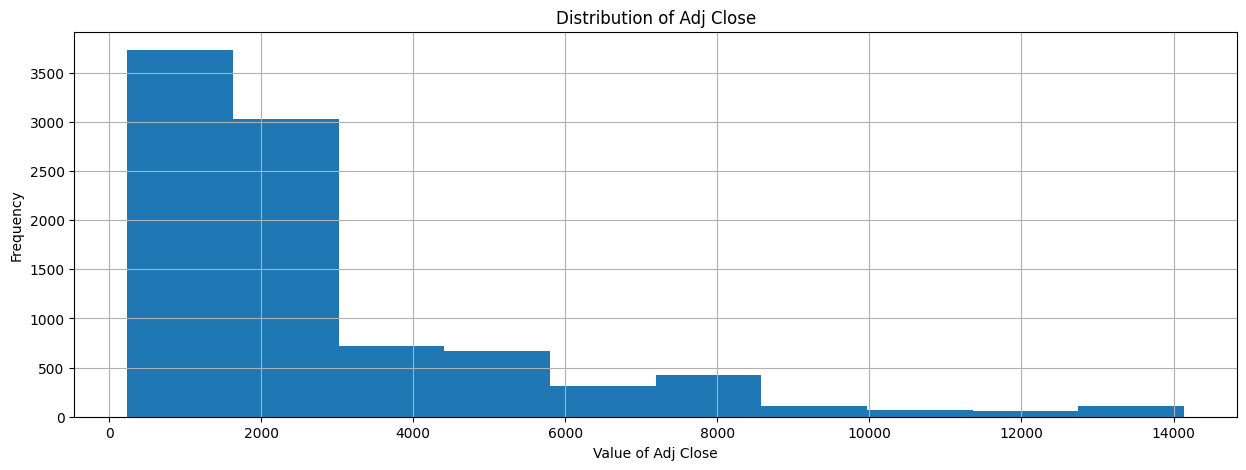
\includegraphics[width=1\textwidth]{Distribution of Adjusted Close.png}
        \caption{Distribution of Open, Low, High, and Adjusted Close in Dataset}
    \end{center}
\end{figure}

Meanwhile, the graph of daily volume traded over time shows that market activity has increased over time, which can be attributed to the rise of electronic trading making the stock market more accessible to everyone, including high-frequency trading firms.

\begin{figure}[H]
    \begin{center}
        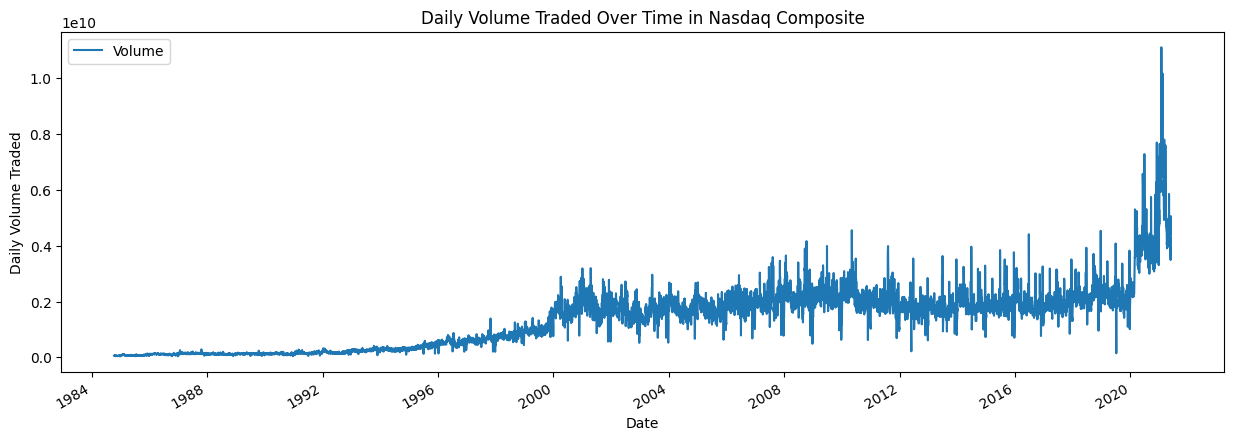
\includegraphics[width=1\textwidth]{Daily Volume Traded Over Time in Nasdaq Composite.png}
        \caption{Daily Volume Traded Over Time in Nasdaq Composite}
    \end{center}
\end{figure}

I also used Pearson's correlation coefficient to find the correlation between features and the adjusted close price, which is our target variable. As expected, the low, high, and open prices are highly correlated with the adjusted close price because they represent the variance of the index's price over the day. Volume appears to be correlated to adjusted close price, but not as strongly as the other features. However, it is difficult to draw conclusions from this as correlation does not imply causation.

\begin{figure}[H]
    \begin{center}
        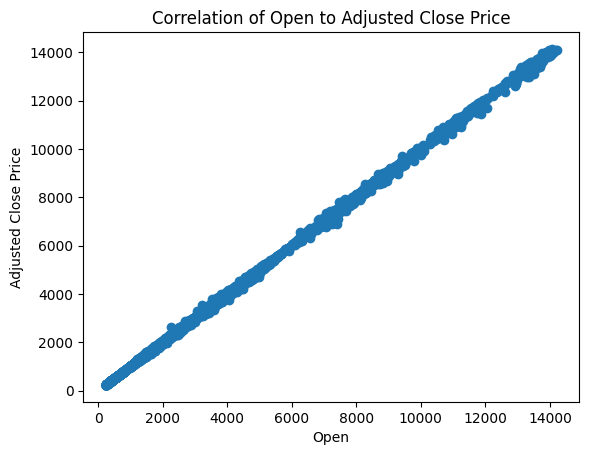
\includegraphics[width=0.6\textwidth]{Correlation of Open to Adjusted Close Price.png}
        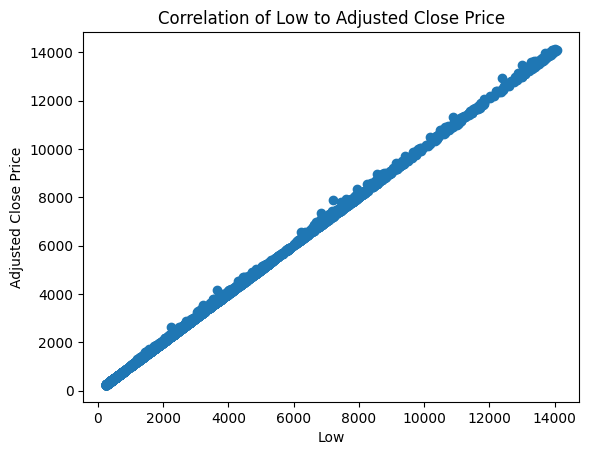
\includegraphics[width=0.6\textwidth]{Correlation of Low to Adjusted Close Price.png}
        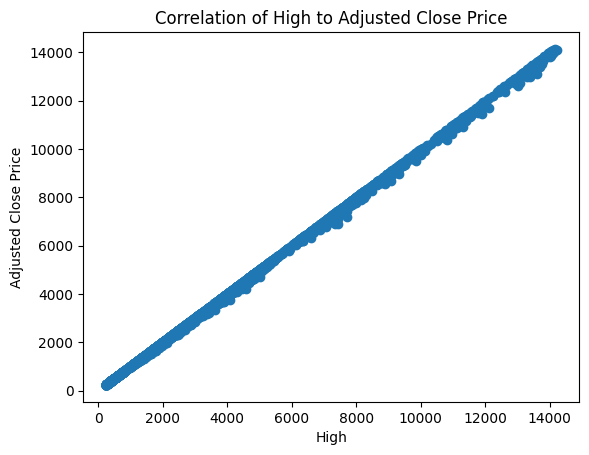
\includegraphics[width=0.6\textwidth]{Correlation of High to Adjusted Close Price.png}
        \caption{Correlation of Open, Low, and High against Adjusted Close in Nasdaq Composite}
    \end{center}
\end{figure}

\begin{figure}[H]
    \begin{center}
        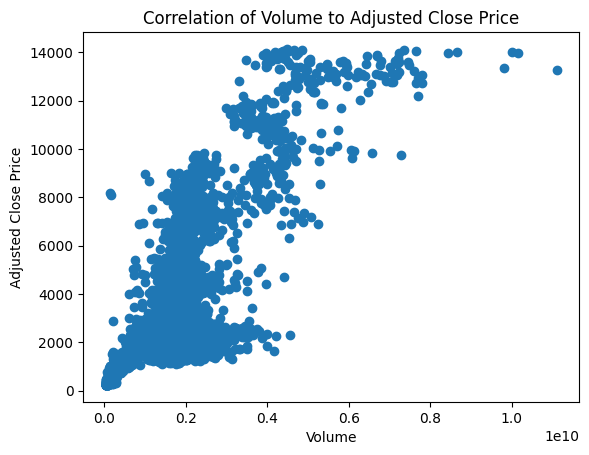
\includegraphics[width=0.6\textwidth]{Correlation of Volume to Adjusted Close Price.png}
        \caption{Correlation of Volume against Adjusted Close in Nasdaq Composite}
    \end{center}
\end{figure}


\subsection{Feature Engineering}
The moving average is a data smoothing technique that is used to track price movements by plotting the average prices over a period of time \cite{movingAverageChart}. It helps to  remove noise from random short-term price fluctuations in data to highlight the overall trend direction \cite{movingAverageChart}.

Simple moving averages give equal weight to each point, whereas exponential moving averages give more weight to recent points. Choosing the time period is a trade-off between noise and accuracy -- a longer period will smooth out the data more, but it will also be less accurate. I applied these techniques on each index to show how it works with different price patterns.

\subsection{Data Filtering}
I compared the simple and exponential moving averages over 30, 90, and 360 day periods on the IXIC data. The 360 day simple and exponential moving averages were poor indicators of the adjusted close price, as they lost too much information and tracked price movements poorly. Thus, I removed them from the dataset and focused on the 30 day and 90 day exponential and simple moving averages.

\begin{figure}[H]
    \begin{center}
        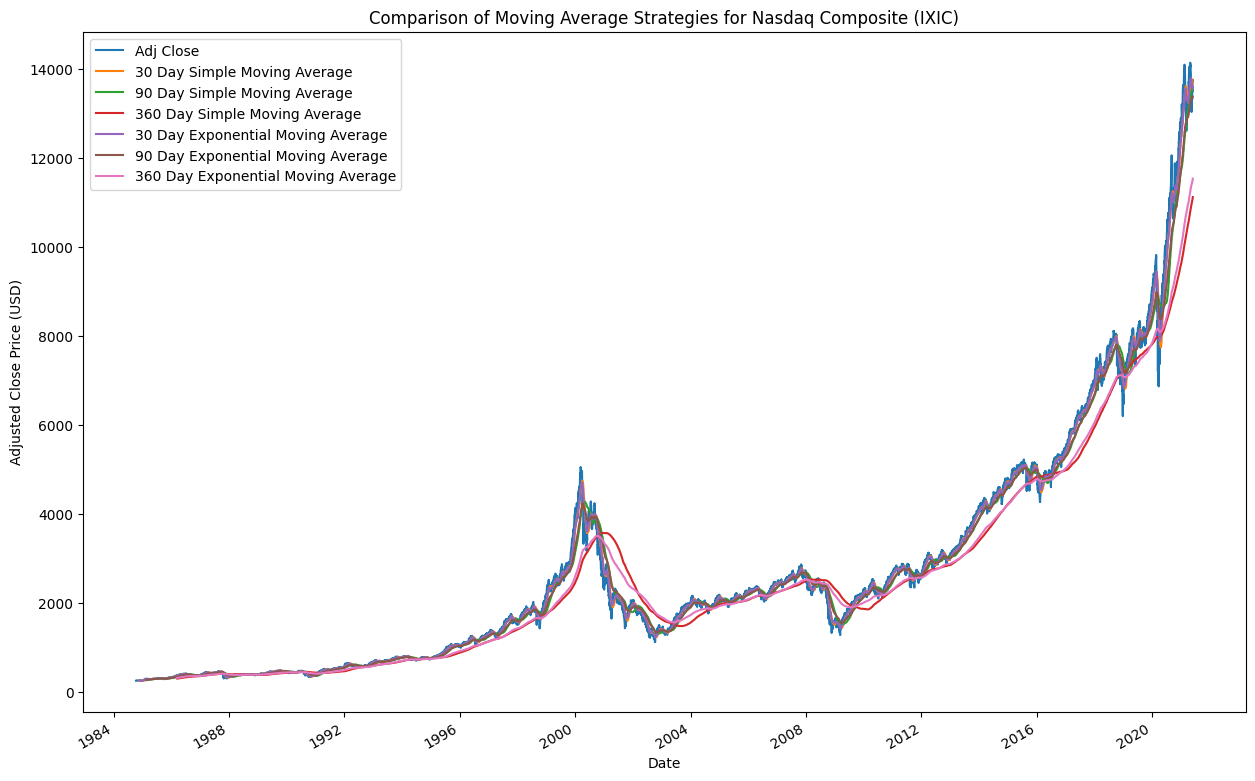
\includegraphics[width=1\textwidth]{Comparison of Moving Average Strategies for Nasdaq Composite.png}
        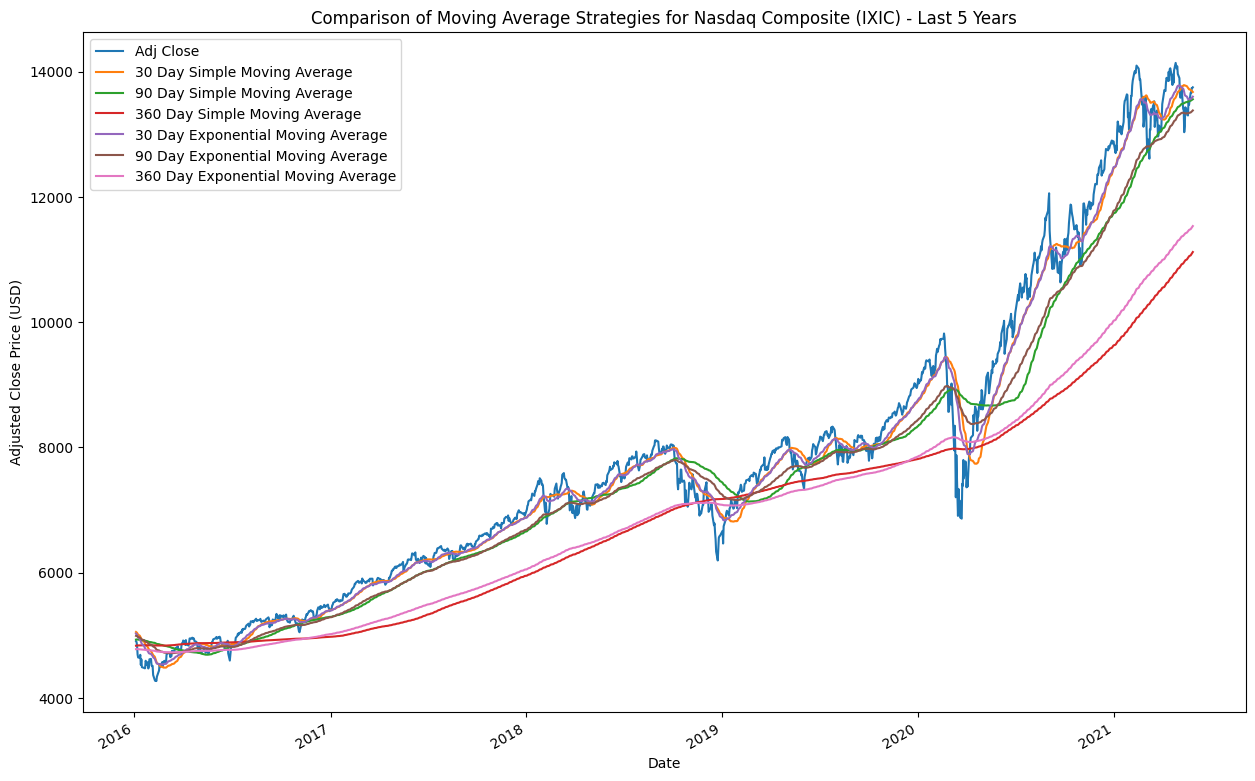
\includegraphics[width=1\textwidth]{Comparison of Moving Average Strategies for Nasdaq Composite (Last 5 Years).png}
        \caption{Comparison of Moving Average Strategies for Nasdaq Composite}
    \end{center}
\end{figure}

\subsection{Data Preprocessing}
I decided to focus on predicting the adjusted close price 30 days in advance, as this would be useful to institutional investors who want to invest part of their monthly paycheck. Thus, I shifted the values of my four input variables to the future by 30 days.

Then, I split the data into training and testing sets, with 80\% of the data being used for training and 20\% for testing. The training set will be used train the regression models and the testing set will be used to evaluate their performance.

\subsection{Regression Models}
I will apply three different regression models to generate price predictions and compare their performance.

Ridge regression is a regularised linear regression model that uses L2 regularization to reduce the variance of the model. It is useful for reducing overfitting and improving the generalisation of the model.

LASSO regression is another regularised linear regression model that uses L1 regularization to reduce the variance of the model. It is useful for feature selection, as it can remove features that are not important to the model.

Polynomial regression is a linear regression model that uses polynomial features to fit a non-linear relationship between the input and target variables.

\subsection{Model Evaluation}
For each regression model, I will calculate the $R^2$ score, which is the proportion of the variance in the target variable that is predictable from the input variable. The closer the $R^2$ score is to 1.0, the better the model is at predicting the target variable. We will compare this score to the $R^2$ score of the naive benchmark that simply predicts adjusted close price based on the last price of the index.

\section{Results}
\subsection{Ridge Regression}
I performed hyperparameter tuning on the ridge regression model using grid search with 5-fold cross validation on several values of alpha between 0.1 and 1000.0. I found the optimal alpha value was 0.1, achieving a mean test score of 0.652964, although the mean test score varied very little between alpha values.

With an alpha value of 0.1, ridge regression achieved an $R^2$ score of 0.95623 when predicting on the test set.

\begin{figure}[H]
    \begin{center}
        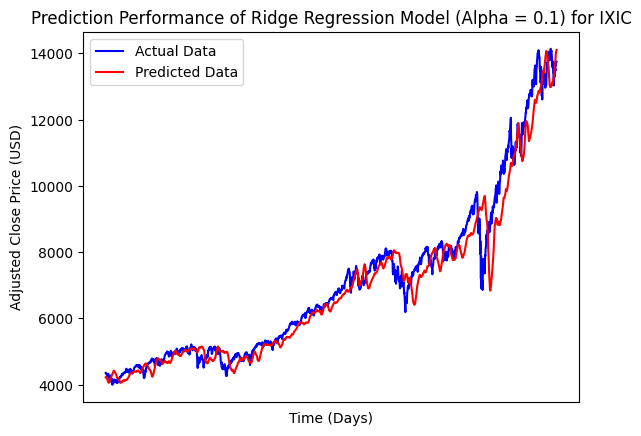
\includegraphics[width=1\textwidth]{Prediction Performance of Ridge Regression Model.png}
        \caption{Prediction Performance of Ridge Regression Model}
    \end{center}
\end{figure}

\subsection{LASSO Regression}
The hyperparameter tuning for the LASSO regression model was performed in the same way, with alpha values ranging from 0.1 to 1000.0. However, the mean test scores varied a lot more, and I found the optimal alpha value to be 1000.0, achieving a mean test score of 0.616147.

With an alpha value of 1000.0, LASSO regression achieved an $R^2$ score of 0.95243 when predicting on the test set, which was slightly worse than ridge regression. Both ridge and LASSO are regularised linear regression models, so it is not surprising that they performed similarly.

\begin{figure}[H]
    \begin{center}
        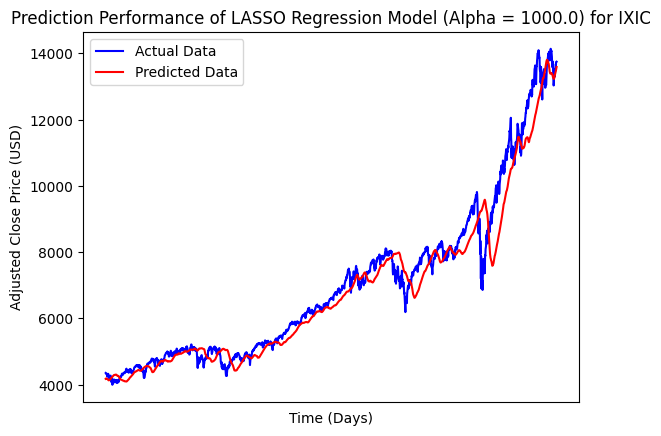
\includegraphics[width=1\textwidth]{Prediction Performance of LASSO Regression Model.png}
        \caption{Prediction Performance of LASSO Regression Model}
    \end{center}
\end{figure}

\subsection{Polynomial Regression}
For the polynomial regression model, I used a pipeline to apply polynomial features to the input variables before fitting the model. I performed hyperparameter tuning on the degree of the polynomial features, testing each degree between 2 and 8. I found the optimal degree to be 2, achieving a mean test score of 0.804763.

Polynomial regression performed poorly, achieving a $R^2$ score of only 0.57730 on the test set. This was significantly worse than the other two models, which suggests that there is a linear relationship between the input and target variables.

\begin{figure}[H]
    \begin{center}
        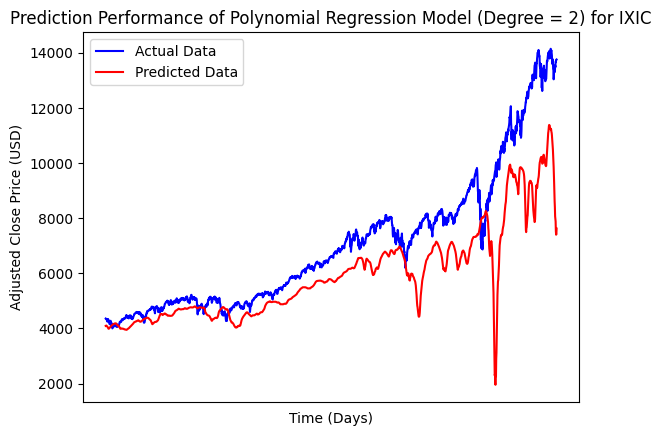
\includegraphics[width=1\textwidth]{Prediction Performance of Polynomial Regression Model.png}
        \caption{Prediction Performance of Polynomial Regression Model}
    \end{center}
\end{figure}

\section{Discussion}

\subsection{Comparison to Last Value Naive Benchmark}
To evaluate the usefulness of our results, we implemented the last value benchmark, which predicts the adjusted close price 30 days in advance by simply using the last value of the adjusted close price. It performed slightly better than our models, achieving an $R^2$ score of 0.96029. This suggests that our models are ineffective at forecasting prices on the Nasdaq Composite Index. However, it may still be useful to predict general trends -- whereas the last value benchmark has a consistent lagging sentiment, our models may be able to predict when the sentiment is changing.

\begin{figure}[H]
    \begin{center}
        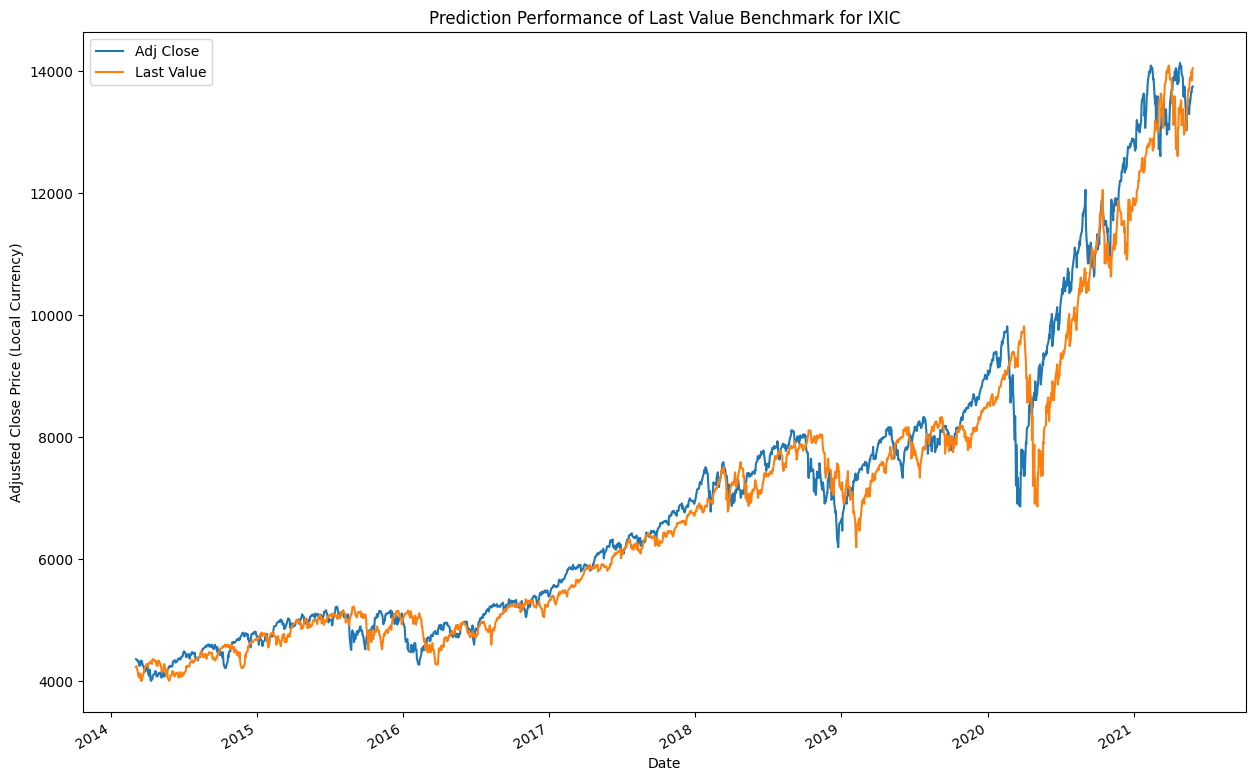
\includegraphics[width=1\textwidth]{Prediction Performance of Last Value Benchmark.png}
        \caption{Prediction Performance of Last Value Benchmark}
    \end{center}
\end{figure}

\subsection{Limitations of the Study and Future Work}
The efficient market hypothesis states that asset prices reflect all available information, which makes it difficult to get arbitrage opportunities. However, Renaissance Technologies, a hedge fund that uses systematic methods, serves as a perfect counter-example -- their Medallion Fund has achieved 66.07\% annualised returns since 1988 \cite{cornell2020medallion}. This suggests that it may be possible to achieve better results with higher quality data. Examples of this include data on a minute by minute basis rather than daily and the number of buy and sell orders on the market.

Furthermore, the stock market involves game theory between market participants -- prices are an equilibrium between people going long and short, so any signals that provide good predictions for future prices will be quickly discovered and priced in. This means that models that are successful on backtested data are unlikely to be successful in the future.

Future analysis could focus on logarithmic returns as the target variable -- this may be a more relevant measure for investors, as they represent relative changes in prices rather than absolute changes, they are symmetric, and they are additive over time \cite{whyLogReturns}. These factors could make it easier to make predictions with a regression model.

\begin{figure}[H]
    \begin{center}
        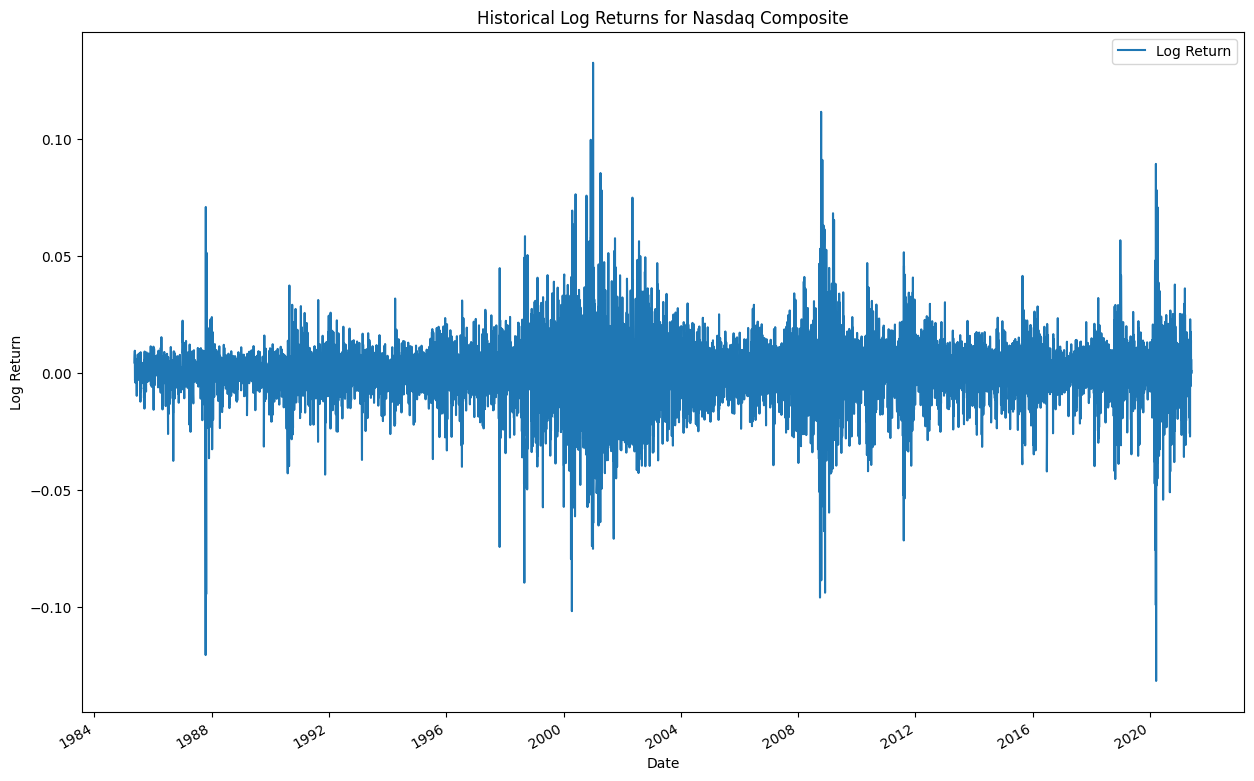
\includegraphics[width=1\textwidth]{Historical Log Returns for Nasdaq Composite.png}
        \caption{Historical Log Returns for Nasdaq Composite}
    \end{center}
\end{figure}

\bibliography{main}
\bibliographystyle{ieeetr.bst}

\end{document}